\documentclass{amsart}

\usepackage[T1]{fontenc}
\usepackage{enumerate, amsmath, amsfonts, amssymb, amsthm, mathrsfs, wasysym, graphics, graphicx, xcolor, url, hyperref, hypcap, xargs, multicol, pdflscape, multirow, hvfloat, array, ae, aecompl, pifont, mathtools, a4wide, float, blkarray, overpic, nicefrac}
\usepackage[noabbrev,capitalise]{cleveref}
\usepackage[normalem]{ulem}
\usepackage{marginnote}
\hypersetup{colorlinks=true, citecolor=darkblue, linkcolor=darkblue}
\usepackage[all]{xy}
\usepackage{tikz}
\usepackage{tikz-cd}
\usepackage{tkz-graph}
\usetikzlibrary{trees, decorations, decorations.pathmorphing, decorations.markings, decorations.shapes, shapes, arrows, matrix, calc, fit, intersections, patterns, angles}
\graphicspath{{figures/}{figures/diagonals/}{figures/walks/}{figures/tubes/}}
\makeatletter\def\input@path{{figures/}}\makeatother
\usepackage{caption}
\captionsetup{width=\textwidth}
\usepackage[export]{adjustbox}

%%%%%%%%%%%%%%%%%%%%%%%%%%%%%%%%%%%%%%

% theorems
\newtheorem{theorem}{Theorem}[section]
\newtheorem{corollary}[theorem]{Corollary}
\newtheorem{proposition}[theorem]{Proposition}
\newtheorem{lemma}[theorem]{Lemma}
\newtheorem{conjecture}[theorem]{Conjecture}
\newtheorem*{theorem*}{Theorem}%[section]

\theoremstyle{definition}
\newtheorem{definition}[theorem]{Definition}
\newtheorem{example}[theorem]{Example}
\newtheorem{remark}[theorem]{Remark}
\newtheorem{question}[theorem]{Question}
\newtheorem{notation}[theorem]{Notation}
\newtheorem{assumption}[theorem]{Assumption}
\newtheorem{convention}[theorem]{Convention}

\crefname{equation}{Equation}{Equations}

% math special letters
\newcommand{\R}{\mathbb{R}} % reals
\newcommand{\Q}{\mathbb{Q}} % rationals
\newcommand{\N}{\mathbb{N}} % naturals
\newcommand{\Z}{\mathbb{Z}} % integers
\newcommand{\C}{\mathbb{C}} % complex
\newcommand{\I}{\mathbb{I}} % set of integers
\newcommand{\HH}{\mathbb{H}} % hyperplane
\newcommand{\K}{k} % field
\newcommand{\f}[1]{{\mathfrak{#1}}} % mathfrak letters
\newcommand{\cal}[1]{{\mathcal{#1}}} % call letters
\renewcommand{\b}[1]{{\boldsymbol{#1}}} % bold letters
\newcommand{\h}{\widehat} % hat letters

% math commands
\newcommand{\set}[2]{\left\{ #1 \;\middle|\; #2 \right\}} % set notation
\newcommand{\bigset}[2]{\big\{ #1 \;\big|\; #2 \big\}} % big set notation
\newcommand{\Bigset}[2]{\Big\{ #1 \;\Big|\; #2 \Big\}} % Big set notation
\newcommand{\setangle}[2]{\left\langle #1 \;\middle|\; #2 \right\rangle} % set notation
\newcommand{\ssm}{\smallsetminus} % small set minus
\newcommand{\dotprod}[2]{\left\langle \, #1 \; \middle| \; #2 \, \right\rangle} % dot product
\newcommand{\bigdotprod}[2]{\big\langle \, #1 \; \big| \; #2 \, \big\rangle} % dot product
\newcommand{\symdif}{\,\triangle\,} % symmetric difference
\newcommand{\one}{{1\!\!1}} % the all one vector
\newcommand{\eqdef}{\mbox{\,\raisebox{0.2ex}{\scriptsize\ensuremath{\mathrm:}}\ensuremath{=}\,}} % :=
\newcommand{\defeq}{\mbox{~\ensuremath{=}\raisebox{0.2ex}{\scriptsize\ensuremath{\mathrm:}} }} % =:
\newcommand{\simplex}{\triangle} % simplex
\renewcommand{\implies}{\Rightarrow} % imply sign
\newcommand{\transpose}[1]{{#1}^T} % transpose matrix

% operators
\DeclareMathOperator{\conv}{conv} % convex hull
\DeclareMathOperator{\vect}{vect} % linear span
\DeclareMathOperator{\cone}{cone} % cone hull

% others
\newcommand{\ie}{\textit{i.e.}~} % id est
\newcommand{\eg}{\textit{e.g.}~} % exempli gratia
\newcommand{\Eg}{\textit{E.g.}~} % exempli gratia
\newcommand{\apriori}{\textit{a priori}} % a priori
\newcommand{\viceversa}{\textit{vice versa}} % vice versa
\newcommand{\versus}{\textit{vs.}~} % versus
\newcommand{\aka}{\textit{a.k.a.}~} % also known as
\newcommand{\perse}{\textit{per se}} % per se
\newcommand{\ordinal}{\textsuperscript{th}} % th for ordinals
\newcommand{\ordinalst}{\textsuperscript{st}} % st for ordinals
\definecolor{darkblue}{rgb}{0,0,0.7} % darkblue color
\definecolor{green}{RGB}{57,181,74} % green color
\definecolor{violet}{RGB}{147,39,143} % violet color
\newcommand{\red}{\color{red}} % red command
\newcommand{\blue}{\color{blue}} % blue command
\newcommand{\orange}{\color{orange}} % orange command
\newcommand{\green}{\color{green}} % green command
\newcommand{\darkblue}{\color{darkblue}} % darkblue command
\newcommand{\defn}[1]{\textsl{\darkblue #1}} % emphasis of a definition
\newcommand{\para}[1]{\medskip\noindent\uline{\textit{#1.}}} % paragraph
\renewcommand{\topfraction}{1} % possibility to have one page of pictures
\renewcommand{\bottomfraction}{1} % possibility to have one page of pictures
\newcommand{\ex}{_{\textrm{exm}}} % examples
\newcommand{\pa}{_{\textrm{pa}}} % path
\newcommand*\circled[1]{\tikz[baseline=(char.base)]{\node[shape=circle, draw, inner sep=1.5pt, scale=.7] (char) {#1};}}
\newcommand{\compactVectorD}[2]{\begin{bmatrix} #1 \\ #2 \end{bmatrix}}
\newcommand{\compactVectorT}[3]{\begin{bmatrix} #1 \\[-.1cm] #2 \\[-.1cm] #3 \end{bmatrix}}

% marginal comments
\usepackage{todonotes}
\newcommand{\arnau}[1]{\todo[color=orange!30]{#1 --- A.}}
\newcommand{\yann}[1]{\todo[color=red!30]{#1 --- Y.}}
\newcommand{\vincent}[1]{\todo[color=blue!30]{#1 \\ \hfill --- V.}}
\newcommand{\pg}[1]{\todo[color=green!30]{#1 \\ \hfill --- PG.}}

% geometry
\newcommandx{\Asso}[2][1=n,2={}]{\mathsf{Asso}^{#2}(#1)} % associahedron
\newcommandx{\Zono}[2][1=n,2={}]{\mathsf{Zono}^{#2}(#1)} % zonotope
\newcommandx{\Fan}[1][1=F]{\mathcal{#1}} % fan
\newcommand{\multiplicityVector}{\b{m}} % multiplicity vector
\newcommandx{\ray}[1][1=r]{\b{#1}} % ray
\newcommandx{\rays}[1][1=R]{\b{#1}} % rays
\newcommand{\gvector}[1]{\b{g}(#1)} % g-vector of #1
\newcommand{\gvectorFull}[2]{\b{g}(#1,#2)} % g-vector of #2 wrt #1
\newcommand{\gvectors}[1]{\b{g}(#1)} % g-vectors of #1
\newcommand{\gvectorsFull}[2]{\b{g}(#1,#2)} % g-vectors of #2 wrt #1
\newcommandx{\gvectorFan}[1][1=\quiver]{\mathcal{F}(#1)} % g-vector fan
\newcommand{\cvector}[2]{\mathbf{c}(#2 \in #1)} % c-vector of the cluster variable #2 in the cluster #1
\newcommand{\cvectorFull}[3]{\mathbf{c}(#1,#3 \in #2)} % c-vector of the cluster variable #3 in the cluster #2 with respect to the initial cluster #1
\newcommand{\cvectors}[1]{\mathbf{c}(#1)} % c-vectors of the cluster #1
\newcommand{\cvectorsFull}[2]{\mathbf{c}(#1,#2)} % c-vectors of the cluster #2 with respect to the initial cluster #1

% Type cone
\newcommand{\typeCone}{\mathbb{TC}} % type cone
\newcommand{\ctypeCone}{\overline{\mathbb{TC}}} % type cone
\newcommand{\compatibilityDegree}[2]{(#1\,\|\,#2)} % compatibility degree
\newcommandx{\coefficient}[3][1={\ray[s]}, 2=\ray, 3=\ray']{\alpha_{#2,#3}(#1)} % coefficient in linear dependence

% Cluster algebras
\newcommand{\Trop}[1]{\mathbb{P}_{#1}} % tropical semifield
\newcommand{\positiveExponents}[1]{\left\{#1\right\}_+} % positive exponents in tropical semifield
\newcommand{\negativeExponents}[1]{\left\{#1\right\}_-} % negative exponents in tropical semifield
\newcommand{\seed}{\Sigma} % a cluster
\newcommand{\cluster}{\mathrm{X}} % a cluster
\newcommandx{\clusters}{\mathcal{X}} % all clusters
\newcommand{\coefficients}{\mathrm{P}} % a coefficients tuple
\newcommandx{\variables}[2][1=\B_\circ, 2 = \coefficients_\circ]{\mathcal{V}(#1,#2)} % all variables
\newcommandx{\clusterAlgebra}[2][1=\B_\circ, 2=\coefficients_\circ]{\mathcal{A}\!\left(#1,#2\right)} % cluster algebra
\newcommandx{\principalClusterAlgebra}[1][1=\B_\circ]{\mathcal{A}\left(#1\right)} % principal coefficients cluster algebra
\newcommandx{\principalVariables}[1][1=\B_\circ]{\mathcal{V}(#1)} % all variables, principal case
\newcommandx{\coefficientFreeClusterAlgebra}[1][1=\B_\circ]{\mathcal{A}_{\mathrm{fr}}(#1)} % coefficient free cluster algebra
\newcommandx{\clusterComplex}[1][1=\B_\circ]{\Delta(#1)} % cluster complex
\newcommand{\B}{\mathrm{B}} % b-matrix
\newcommand{\A}[1]{\mathrm{A}({#1})} % b-matrix
\newcommand{\D}{\mathrm{D}} % symmetrizer
\newcommand{\simpleRoot}{\alpha} % simple root
\newcommand{\fundamentalWeight}{\omega} % fundamental weights
\newcommandx{\meshes}[1][1=\B_\circ]{\mathcal{M}(#1)} % meshes

% Gentle associahedra
\newcommand{\quiver}{\bar Q} % quiver
\newcommand{\blossom}{^\text{\ding{96}}} % blossom
\newcommandx{\strings}[1][1=\quiver]{\mathcal{S}(#1)} % strings
\newcommandx{\distinguishableStrings}[1][1=\quiver]{\mathcal{S}_\mathrm{dist}(#1)} % distinguishable strings
\newcommandx{\walks}[1][1=\quiver]{\mathcal{W}(#1)} % walks
\newcommandx{\properWalks}[1][1=\quiver]{\mathcal{W}_\mathrm{prop}(#1)} % proper walks
\renewcommand{\top}{\mathrm{top}} % top
\newcommand{\bottom}{\mathrm{bot}} % bottom
\newcommandx{\NKC}[1][1=\quiver]{\mathcal{NK}(#1)} % non-kissing complex
\newcommandx{\RNKC}[1][1=\quiver]{\mathcal{RNK}(#1)} % reduced non-kissing complex
\newcommand{\peaks}[1]{\mathsf{peaks}(#1)} % peaks
\newcommand{\deeps}[1]{\mathsf{deeps}(#1)} % deeps
\newcommand{\KN}{\textsc{kn}} % Kissing Number
\newcommand{\hL}{\text{\rotatebox[origin=c]{180}{\checked}}}
\newcommand{\hR}{\text{\rotatebox[origin=c]{180}{\reflectbox{\checked}}}}
\newcommand{\cL}{\text{\reflectbox{\checked}}}
\newcommand{\cR}{\text{\checked}}
\newcommand{\hh}[1]{\hL#1\hR} % hook - hook
\newcommand{\cc}[1]{\cL#1\cR} % cohook - cohook
\newcommand{\hc}[1]{\hL#1\cR} % hook - cohook
\newcommand{\ch}[1]{\cL#1\hR} % cohook - hook
\newcommand{\distinguishedString}[2]{\mathsf{ds}(#1,#2)} % distinguished string
\newcommand{\distinguishedSign}[2]{\varepsilon(#1,#2)} % distinguished sign

% Graph associahedra
\newcommand{\ground}{V} % ground set
\newcommandx{\graphG}[1][1=G]{#1} % graph
\newcommandx{\tube}[1][1=t]{\mathsf{#1}} % tube
\newcommandx{\tubes}[1][1=\graphG]{\mathcal{T}(#1)} % all tubes
\newcommandx{\tubing}[1][1=T]{\mathsf{#1}} % tubing
\newcommand{\connectedComponents}{\kappa} % connected components
\newcommand{\nestedComplex}{\mathcal{N}} % nested complex
\newcommand{\nonDisconnecting}{\mathrm{nd}} % non-disconnecting vertices
\newcommand{\neighbors}{\mathrm{ne}} % neighbors

% Representation theory
\newcommand{\field}{\mathbb{K}}
\newcommand{\cat}{\mathcal{C}}
\newcommand{\Hom}[1]{\operatorname{Hom}_{#1}}
\newcommand{\susp}{\Sigma}
\newcommand{\add}{\operatorname{add}}
\newcommand{\MOD}{\operatorname{mod}}
\newcommand{\End}[1]{\operatorname{End}_{#1}}
\newcommand{\spl}{\operatorname{sp}}
\newcommand{\Ksp}{K_0^{\spl}}
\newcommand{\Kg}{K_0^{\b{g}}}
\newcommand{\ind}{\operatorname{ind}}
\newcommand{\coker}{\operatorname{coker}}
\newcommand{\CC}{\phi}
\newcommand{\proj}{\operatorname{proj}}
\newcommand{\bsm}{\begin{smallmatrix}}
\newcommand{\esm}{\end{smallmatrix}}

% Extriangulated categories
\newcommand{\tc}{\mathcal{T}}
\newcommand{\ec}{\mathcal{E}}
\newcommand{\infl}{\rightarrowtail}
\newcommand{\defl}{\twoheadrightarrow}
\newcommand{\Modt}{\operatorname{Mod}\tc}
\newcommand{\modt}{\MOD\tc}
\newcommand{\kzero}[1]{K_0(#1)}
\newcommand{\eps}{\varepsilon}

%%%%%%%%%%%%%%%%%%%%%%%%%%%%%%%%%%%%%%

% formating the part command
\makeatletter
\def\part{\@startsection{part}{1}%
\z@{.7\linespacing\@plus\linespacing}{.8\linespacing}%
{\LARGE\sffamily\centering}}
%\@addtoreset{section}{part}
\makeatother
\renewcommand{\thepart}{\Roman{part}}
%\renewcommand{\thesection}{\arabic{part}.\arabic{section}}

% formating the table of contents
\setcounter{tocdepth}{4}
\makeatletter
\def\l@section{\@tocline{1}{5pt}{0pc}{}{}}
\makeatother
\let\oldtocpart=\tocpart
\renewcommand{\tocpart}[2]{\sc\large\oldtocpart{#1}{#2}}
\let\oldtocsection=\tocsection
\renewcommand{\tocsection}[2]{\bf\oldtocsection{#1}{#2}}
\let\oldtocsubsubsection=\tocsubsubsection
\renewcommand{\tocsubsubsection}[2]{\quad\oldtocsubsubsection{#1}{#2}}

%%%%%%%%%%%%%%%%%%%%%%%%%%%%%%%%%%%%%%

\title[The type cone of graph associahedra]{The type cone of graph associahedra}

\thanks{YP, VP and PGP were partially supported by the French ANR grant SC3A~(15\,CE40\,0004\,01). AP and VP were partially supported by the French ANR grant CAPPS~(17\,CE40\,0018).}

\author{Arnau Padrol}
\address[Arnau Padrol]{Institut de Math�matiques de Jussieu - Paris Rive Gauche, Sorbonne Universit\'e, Paris}
\email{arnau.padrol@imj-prg.fr.}
\urladdr{\url{https://webusers.imj-prg.fr/~arnau.padrol/}}

\author{Yann Palu}
\address[Yann Palu]{LAMFA, Universit\'e Picardie Jules Verne, Amiens}
\email{yann.palu@u-picardie.fr}
\urladdr{\url{http://www.lamfa.u-picardie.fr/palu/}}

\author{Vincent Pilaud}
\address[Vincent Pilaud]{CNRS \& LIX, \'Ecole Polytechnique, Palaiseau}
\email{vincent.pilaud@lix.polytechnique.fr}
\urladdr{\url{http://www.lix.polytechnique.fr/~pilaud/}}

\author{Pierre-Guy Plamondon}
\address[Pierre-Guy Plamondon]{Laboratoire de Math\'ematiques d'Orsay, Universit\'e Paris-Sud, CNRS, Universit\'e Paris-Saclay}
\email{pierre-guy.plamondon@math.u-psud.fr}
\urladdr{\url{https://www.math.u-psud.fr/~plamondon/}}

%%%%%%%%%%%%%%%%%%%%%%%%%%%%%%%%%%%%%%

\begin{document}

\begin{abstract}
We give a complete description of the type cone of graph associahedra.
\end{abstract}

\maketitle
% 
% \vspace{1.5cm}
% \centerline{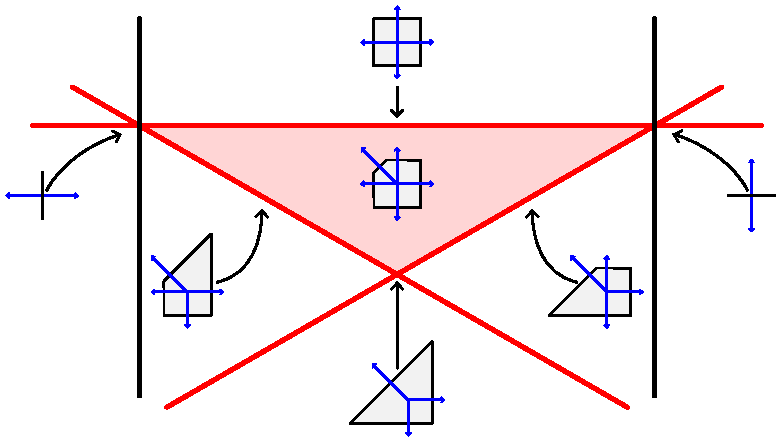
\includegraphics[scale=.8]{typeConeCoarsenings}}
% \vspace{.5cm}
% \centerline{The type cone of the cluster fan of type~$A_2$.}

% \newpage
\tableofcontents

%%%%%%%%%%%%%%%%%%%%%%%%%%%%%%%%%%%%%%%%%%%%%%%%%%%

\newpage
\section*{Introduction}
\arnau{Introduce associahedron}
In~\cite{PPPP}, a new approach for studying the space of polytopal realizations of $\b{g}$-vector fans, based on McMullen's type cones, was introduced to study two generalizations of the associahedron: the generalized associahedra of finite type cluster algebras~\cite{FominZelevinsky-ClusterAlgebrasI, FominZelevinsky-ClusterAlgebrasII, FominZelevinsky-ClusterAlgebrasIV, HohlwegLangeThomas, HohlwegPilaudStella} and the gentle associahedra~\cite{PaluPilaudPlamondon-nonkissing}. 
\arnau{cite physicists and BDMTY}
% This approach sheds a new light on and extends earlier results of N.~Arkani-Hamed, Y.~Bai, S.~He, and G.~Yan in type~$A$ and of V.~Bazier-Matte, G.~Douville, K.~Mousavand, H.~Thomas and E.~Y\i ld\i r\i m for acyclic initial seeds.


It is natural to extend the approach to further families of generalizations of the associahedron. In this paper, we focus on graph associahedra. \textbf{Graph associahedra} were defined by M.~Carr and S.~Devadoss~\cite{CarrDevadoss} in connection to C.~De Concini and C.~Procesi's wonderful arrangements~\cite{DeConciniProcesi}. As illustrated in \cref{fig:specialGraphAssociahedra}, the graph associahedra of certain special families of graphs coincide with well-known families of polytopes: complete graph associahedra are permutahedra, path associahedra are classical associahedra, cycle associahedra are cyclohedra, and star associahedra are stellohedra. The graph associahedra were extended to the nestohedra, which are simple polytopes realizing the nested complex of arbitrary building sets~\cite{Postnikov, FeichtnerSturmfels}. Graph associahedra and nestohedra have been geometrically realized in different ways: by successive truncations of faces of the standard simplex~\cite{CarrDevadoss}, as Minkowski sums of faces of the standard simplex~\cite{Postnikov, FeichtnerSturmfels}, or from their normal fans by exhibiting explicit inequality descriptions~\cite{Devadoss, Zelevinsky}. All these realizations have the same normal fan, called nested fan. 
We study the type cones of these nested fans (see \cref{subsec:typeConeGA}): we describe their facet-defining inequalities in terms of certain specific pairs of neighboring tubings and count them for the specific families of graph associahedra described earlier. For instance the type cone of the permutahedron coincides with the classical submodular functions on~$2^{[n]}$, described by~$2^{n-2} \binom{n}{2}$ inequalities. In fact, we observe that the type cone of a graphical nested fan is never simplicial except in the case of the classical associahedron (when the graph is the path). Nevertheless, our results give a non-redundant description of all polytopal realizations of the graphical nested fans.




\subsection{Graphical nested complexes and graph associahedra}
\label{subsec:typeConeGA}

Graph associahedra were defined by M.~Carr and S.~Devadoss~\cite{CarrDevadoss} in connection to C.~De Concini and C.~Procesi's wonderful arrangements~\cite{DeConciniProcesi}.
For a given graph~$\graphG$, the $\graphG$-associahedron~$\Asso[\graphG]$ is a simple polytope whose combinatorial structure encodes the connected subgraphs of~$\graphG$ and their nested structure.
More precisely, the $\graphG$-associahedron is a polytopal realization of the nested complex of~$\graphG$, defined as the simplicial complex of all collections of tubes (connected induced subgraphs) of~$\graphG$ which are pairwise compatible (either nested, or disjoint and non-adjacent).
As illustrated in \cref{fig:specialGraphAssociahedra}, the graph associahedra of certain special families of graphs coincide with well-known families of polytopes: complete graph associahedra are permutahedra, path associahedra are classical associahedra, cycle associahedra are cyclohedra, and star associahedra are stellohedra.
The graph associahedra were extended to the \defn{nestohedra}, which are simple polytopes realizing the nested complex of arbitrary building sets~\cite{Postnikov, FeichtnerSturmfels}.
Graph associahedra and nestohedra have been geometrically realized in different ways: by successive truncations of faces of the standard simplex~\cite{CarrDevadoss}, as Minkowski sums of faces of the standard simplex~\cite{Postnikov, FeichtnerSturmfels}, or from their normal fans by exhibiting explicit inequality descriptions~\cite{Devadoss, Zelevinsky}.
For a given graph~$\graphG$, the resulting polytopes all have the same normal fan, called nested fan of~$\graphG$: its rays are the characteristic vectors of the tubes, and its cones are generated by characteristic vectors of compatible tubes.
In this section, we describe the type cone of the nested fan of any graph~$\graphG$.

\hvFloat[floatPos=p, capWidth=h, capPos=r, capAngle=90, objectAngle=90, capVPos=c, objectPos=c]{figure}
{
		\begin{tabular}{c@{\;}c@{\;}c@{\;}c}
			permutahedron &
			associahedron &
			cyclohedron &
			stellohedron \\[.2cm]
			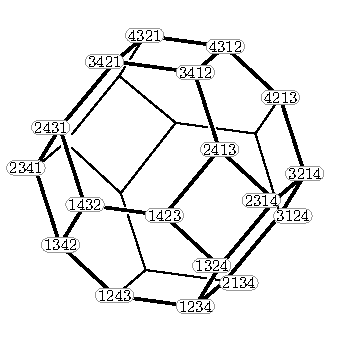
\includegraphics[scale=.93]{permutahedron} &
			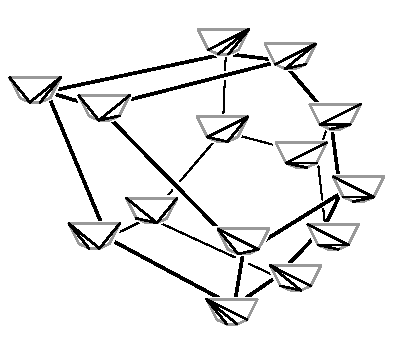
\includegraphics[scale=.93]{associahedron} &
			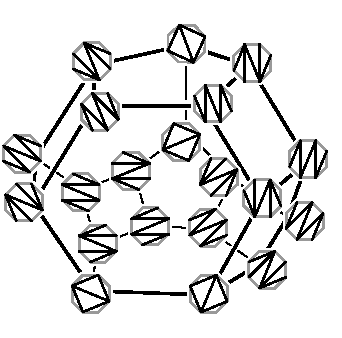
\includegraphics[scale=.93]{cyclohedron} &
			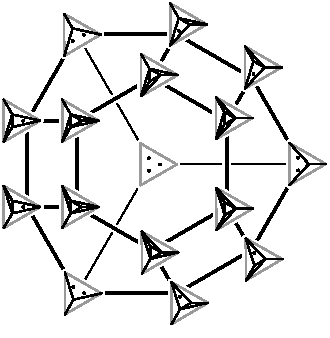
\includegraphics[scale=.93]{stellohedron} \\[.1cm]
			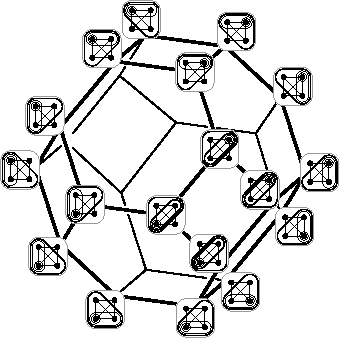
\includegraphics[scale=.93]{permutahedronTubings} &
			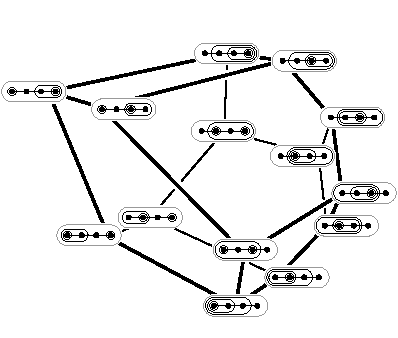
\includegraphics[scale=.93]{associahedronTubings} &
			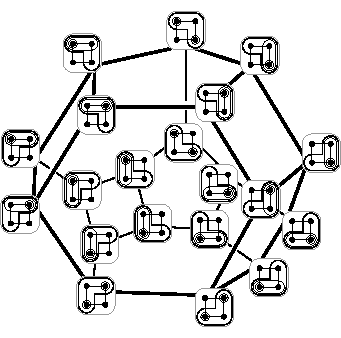
\includegraphics[scale=.93]{cyclohedronTubings} &
			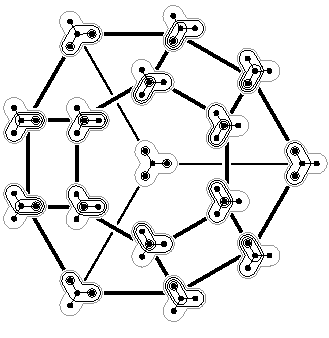
\includegraphics[scale=.93]{stellohedronTubings} \\[.2cm]
			complete graph &
			path &
			cycle &
			star \\[.3cm]
		\end{tabular}
}
{Some classical families of polytopes as graph associahedra. Illustration from~\cite{MannevillePilaud-compatibilityFans}.}
{fig:specialGraphAssociahedra}

%\begin{figure}[t]
%	\capstart
%	\begin{adjustbox}{center}
%		\begin{tabular}{c@{\;}c@{\;}c@{\;}c}
%			permutahedron &
%			associahedron &
%			cyclohedron &
%			stellohedron \\
%			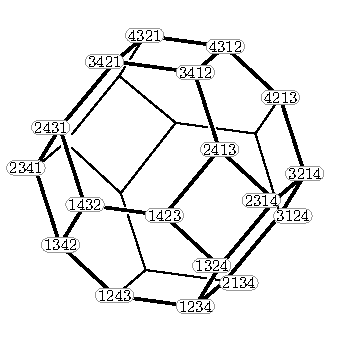
\includegraphics[scale=.6]{permutahedron} &
%			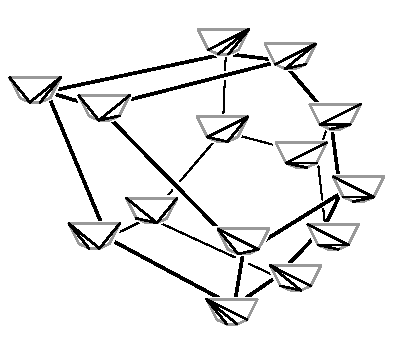
\includegraphics[scale=.6]{associahedron} &
%			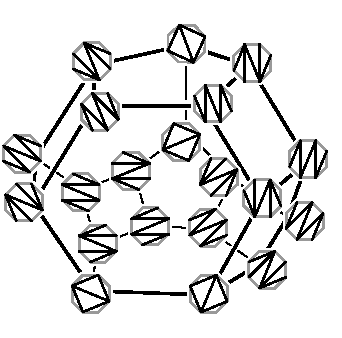
\includegraphics[scale=.6]{cyclohedron} &
%			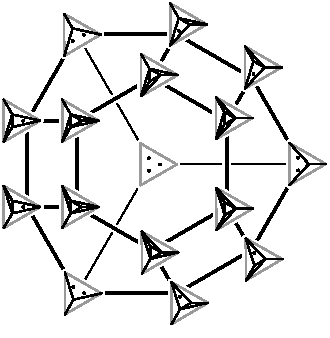
\includegraphics[scale=.6]{stellohedron} \\
%			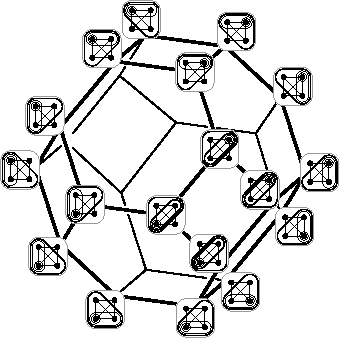
\includegraphics[scale=.6]{permutahedronTubings} &
%			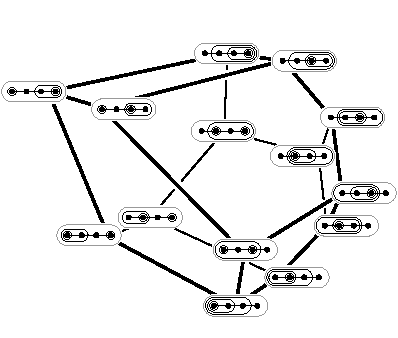
\includegraphics[scale=.6]{associahedronTubings} &
%			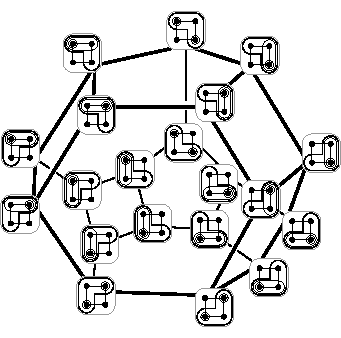
\includegraphics[scale=.6]{cyclohedronTubings} &
%			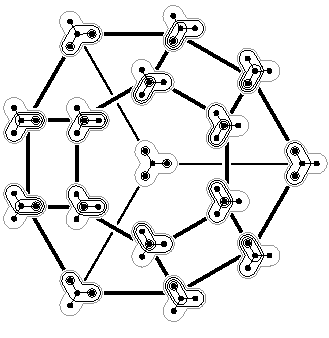
\includegraphics[scale=.6]{stellohedronTubings} \\[.1cm]
%			complete graph &
%			path &
%			cycle &
%			star
%		\end{tabular}
%	\end{adjustbox}
%	\caption{Some classical families of polytopes as graph associahedra. Illustration from~\cite{MannevillePilaud-compatibilityFans}.}
%	\label{fig:specialGraphAssociahedra}
%\end{figure}

%%%

\clearpage
\subsubsection{Nested complex and nested fan of a graph}

We present the definitions and properties of the nested complex of a graph, following ideas from~\cite{CarrDevadoss, Postnikov, FeichtnerSturmfels, Zelevinsky}.

\para{Nested complex}
%
Let~$\graphG$ be a graph with vertex set~$\ground$.
Let~$\connectedComponents(\graphG)$ denote the set of connected components of~$\graphG$ and define~$n \eqdef |\ground|-|\connectedComponents(\graphG)|$.
A \defn{tube} of~$\graphG$ is a subset of vertices of~$\graphG$ whose induced subgraph is connected.
The set of tubes of~$\graphG$ is denoted by~$\tubes$.
The inclusion maximal tubes of~$\graphG$ are its connected components~$\connectedComponents(\graphG)$.
The tubes which are neither empty nor maximal are called \defn{proper}.
Two tubes~$\tube, \tube'$ of~$\graphG$ are \defn{compatible} if they are either nested (\ie $\tube \subseteq \tube'$ or~$\tube' \subseteq \tube$), or disjoint and non-adjacent (\ie $\tube \cup \tube'$ is not a tube of~$\graphG$).
A \defn{tubing} on~$\graphG$ is a set~$\tubing$ of pairwise compatible proper tubes of~$\graphG$.
See \cref{fig:exmNested}.
The \defn{nested complex} of~$\graphG$ is the simplicial complex~$\nestedComplex(\graphG)$ of all tubings~on~$\graphG$.

\begin{figure}[t]
	\capstart
	\centerline{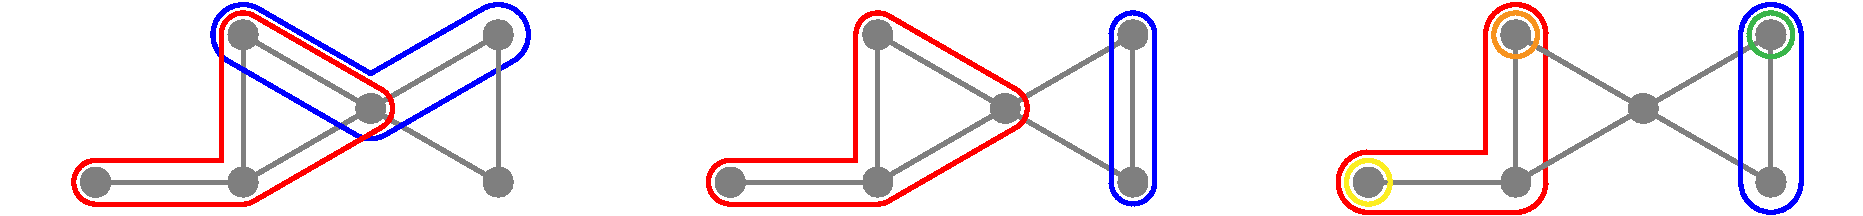
\includegraphics[width=\textwidth]{exmNested}}
	\caption{Some incompatible tubes (left and middle), and a maximal tubing (right).}
	\label{fig:exmNested}
\end{figure}

\para{Nested fan and graph associahedron}
%
Let~$(\b{e}_v)_{v \in \ground}$ be the canonical basis of~$\R^\ground$.
We consider the hyperplane~${\HH \eqdef \bigset{\b{x} \in \R^\ground}{\sum_{w \in W} x_w = 0 \text{ for all } W \in \connectedComponents(\graphG)}}$ and let~$\pi : \R^\ground \to \HH$ denote the orthogonal projection on~$\HH$.

\begin{definition}
The \defn{$\b{g}$-vector} of a tube~$\tube$ of~$\graphG$ is the projection~$\gvector{\tube} \eqdef \pi \big( \sum_{v \in \tube} \b{e}_v \big)$ of the characteristic vector of~$\tube$.
We set~$\gvectors{\tubing} \eqdef \set{\gvector{\tube}}{\tube \in \tubing}$ for a tubing~$\tubing$ on~$\graphG$.
\end{definition}

Note that by definition, $\gvector{\varnothing} = 0$ and $\gvector{W} = 0$ for all connected components~$W \in \connectedComponents(\graphG)$.
These vectors support a complete simplicial fan realization of the nested complex.
Examples are illustrated in \cref{fig:nestedFans}.

\begin{figure}[b]
	\capstart
	\centerline{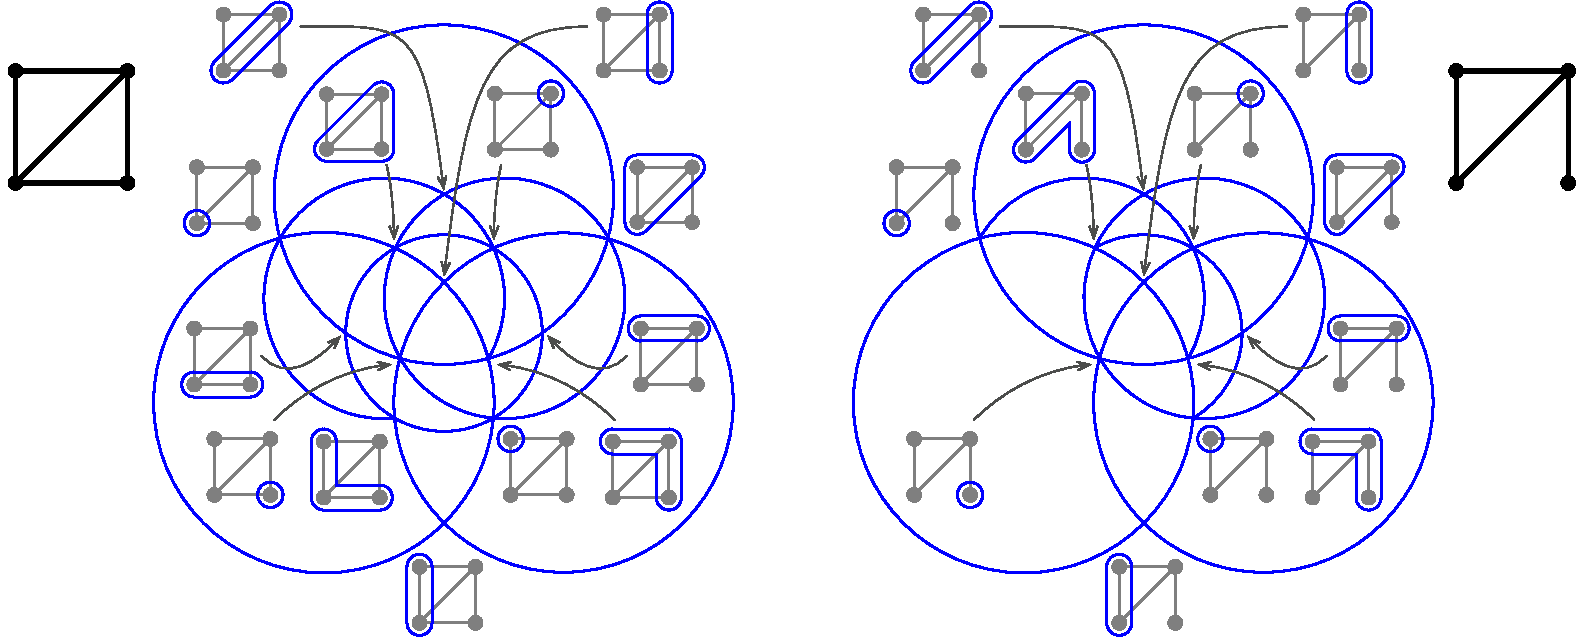
\includegraphics[scale=.55]{nestedFans}}
	\caption{Two nested fans. As the fans are $3$-dimensional, we intersect them with the sphere and stereographically project them from the direction~$(-1,-1,-1)$.}
	\label{fig:nestedFans}
\end{figure}

\begin{theorem}[\cite{CarrDevadoss, Postnikov, FeichtnerSturmfels, Zelevinsky}]
\label{thm:nestedFan}
For any graph~$\graphG$, the set of cones
\[
\gvectorFan[\graphG] \eqdef \set{\R_{\ge 0} \, \gvectors{\tubing}}{\tubing \text{ tubing on } \graphG}
\]
is a complete simplicial fan of~$\HH$, called \defn{nested fan} of~$\graphG$, which realizes the nested complex~$\nestedComplex(\graphG)$.
\end{theorem}

It is proved in~\cite{CarrDevadoss, Devadoss, Postnikov, FeichtnerSturmfels, Zelevinsky} that the nested fan comes from a polytope.
For any subset~$U \subseteq \ground$, denote by~$\triangle_U \eqdef \conv\set{\b{e}_u}{u \in U}$ the face of the standard simplex~$\triangle_\ground$ corresponding to~$U$.

\begin{theorem}[\cite{CarrDevadoss, Devadoss, Postnikov, FeichtnerSturmfels, Zelevinsky}]
For any graph~$\graphG$, the nested fan~$\gvectorFan[\graphG]$ is the normal fan of the graph associahedron~$\Asso[\graphG]$.
It can be constructed as
\begin{itemize}
\item the intersection of~$\HH$ with the hyperplanes~$\dotprod{\gvector{\tube}}{\b{x}} \le 3^{|\tube|-2}$ for all tubes~$\tube \in \tubes$~\cite{Devadoss},
\item the Minkowski sum~$\sum_{\tube \in \tubes} \triangle_{\tube}$ of the faces of the standard simplex corresponding to all tubes of~$\graphG$~\cite{Postnikov}.
\end{itemize}
\end{theorem}

\para{Flips in the nested fan}
%
The following statement follows from~\cite{MannevillePilaud-compatibilityFans, Zelevinsky}.

\begin{proposition}
\label{prop:exchangeablePairsGA}
Let~$\tube, \tube'$ be two tubes of~$\graphG$. Then
\begin{enumerate}[(i)]
\item The tubes~$\tube$ and~$\tube'$ are exchangeable if and only if $\tube'$ has a unique neighbor~$v$ in~$\tube \ssm \tube'$ and $\tube$ has a unique neighbor~$v'$ in~$\tube' \ssm \tube$.
\item For any maximal tubings~$\tubing, \tubing'$ on~$\graphG$ with $\tubing \ssm \{\tube\} = \tubing' \ssm \{\tube'\}$, both~$\tubing \cup \connectedComponents(\graphG)$ and~$\tubing' \cup \connectedComponents(\graphG)$ contain the tube~$\tube \cup \tube'$ and the connected components of~$\tube \cap \tube'$.
\item The linear dependence between the $\b{g}$-vectors of~$\tubing \cup \tubing'$ is given by
\[
\gvector{\tube} + \gvector{\tube'} = \gvector{\tube \cup \tube'} + \sum_{\tube[s] \in \connectedComponents(\tube \cap \tube')} \gvector{\tube[s]}.
\]
\item The nested fan of~$\graphG$ has the unique exchange relation property.
\item The $\b{c}$-vector orthogonal to all $\b{g}$-vectors~$\gvector{\tube[s]}$ for~$\tube[s] \in \tubing \cap \tubing'$ is~$\b{e}_v - \b{e}_{v'}$.
\end{enumerate}
\end{proposition}

\begin{proof}
Points~(i) and~(ii) was proved in~\cite{MannevillePilaud-compatibilityFans}. Point~(iii) follows from the fact that
\[
\sum_{v \in \tube} \b{e}_v + \sum_{v \in \tube'} \b{e}_v = \sum_{v \in \tube \cup \tube'} \b{e}_v + \sum_{v \in \tube \cap \tube'} \b{e}_v = \sum_{v \in \tube \cup \tube'} \b{e}_v + \sum_{\substack{\tube[s] \in \connectedComponents(\tube \cap \tube') \\ v \in \tube[s]}} \b{e}_v.
\]
Point~(iv) is obtained by combining~(ii) and~(iii).
Finally for~(v), any tube~$\tube[s] \in \tubing \cap \tubing'$ that contains~$v$ or~$v'$ actually contains both (to be compatible with~$\tube$ and~$\tube'$). Therefore, $\gvector{\tube[s]}$ is orthogonal to~$\b{e}_v - \b{e}_{v'}$ for any tube~$\tube[s] \in \tubing \cap \tubing'$.
\end{proof}

%%%

\subsubsection{Type cones of graphical nested fans}

We now discuss the type cones of the graphical nested fans defined in \cref{thm:nestedFan}.
We first obtain from \cref{prop:exchangeablePairsGA} the following redundant description.

\begin{corollary}
\label{coro:typeConeGA}
For any graph~$\graphG$, the type cone of the nested fan~$\gvectorFan[\graphG]$ is given by
\[
\typeCone \big( \gvectorFan[\graphG] \big) = \set{\b{h} \in \R^{\tubes}}{\begin{array}{l} \b{h}_{\tube} = 0 \text{ for any improper tube } \tube \\ \b{h}_{\tube} + \b{h}_{\tube'} > \b{h}_{\tube \cup \tube'} + \sum_{\tube[s] \in \connectedComponents(\tube \cap \tube')} \b{h}_{\tube[s]} \text{ for any exchangeable tubes } \tube, \tube' \end{array}}.
\]
\end{corollary}

\begin{example}
For the complete graph~$\graphG[K]_n$, the admissible height vectors are precisely the submodular functions, \ie the functions~$\b{h} : 2^{[n]} \to \R$ such that~$\b{h}_{\varnothing} = 0$ and~$\b{h}_{A} + \b{h}_{B} > \b{h}_{A \cap B} + \b{h}_{A \cup B}$ for any~$A, B \subseteq [n]$.
This is precisely the description of the generalized permutahedra introduced by A.~Postnikov in~\cite{Postnikov} and E.-M.~Feichtner and B.~Sturmfels in~\cite{FeichtnerSturmfels}.
\end{example}

\begin{example}
\label{exm:typeConeGA}
Consider the nested fans illustrated in \cref{fig:nestedFans}.
The type cone of the left fan lives in~$\R^{13}$, has a linearity space of dimension~$3$ and $19$ facet-defining inequalities (given below). In particular, it is not simplicial.

\medskip
\centerline{$
\begin{array}{r|c@{\;\,}c@{\;\,}c@{\;\,}c@{\;\,}c@{\;\,}c@{\;\,}c@{\;\,}c@{\;\,}c@{\;\,}c@{\;\,}c@{\;\,}c@{\;\,}c}
\text{tubes} & \raisebox{-.4cm}{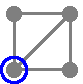
\includegraphics[scale=.6]{tubeA1}} & \raisebox{-.4cm}{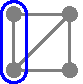
\includegraphics[scale=.6]{tubeA2}} & \raisebox{-.4cm}{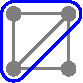
\includegraphics[scale=.6]{tubeA3}} & \raisebox{-.4cm}{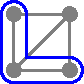
\includegraphics[scale=.6]{tubeA4}} & \raisebox{-.4cm}{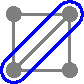
\includegraphics[scale=.6]{tubeA5}} & \raisebox{-.4cm}{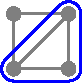
\includegraphics[scale=.6]{tubeA6}} & \raisebox{-.4cm}{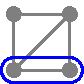
\includegraphics[scale=.6]{tubeA7}} & \raisebox{-.4cm}{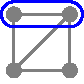
\includegraphics[scale=.6]{tubeA8}} & \raisebox{-.4cm}{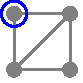
\includegraphics[scale=.6]{tubeA9}} & \raisebox{-.4cm}{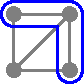
\includegraphics[scale=.6]{tubeA10}} & \raisebox{-.4cm}{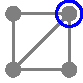
\includegraphics[scale=.6]{tubeA11}} & \raisebox{-.4cm}{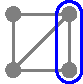
\includegraphics[scale=.6]{tubeA12}} & \raisebox{-.4cm}{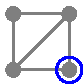
\includegraphics[scale=.6]{tubeA13}}  \\[.6cm]
\text{$\b{g}$-vectors} & \compactVectorT{1}{0}{0} & \compactVectorT{0}{2}{0} & \compactVectorT{0}{0}{1} & \compactVectorT{0}{2}{-1} & \compactVectorT{1}{-2}{1} & \compactVectorT{1}{-2}{0} & \compactVectorT{1}{0}{-1} & \compactVectorT{-1}{2}{0} & \compactVectorT{-1}{0}{1} & \compactVectorT{-1}{0}{0} & \compactVectorT{0}{-2}{1} & \compactVectorT{0}{-2}{0} & \compactVectorT{0}{0}{-1} \\[.6cm]
\text{facet}		& 0 & 0 & 0 & 0 & 0 & 0 & 0 & 0 & 0 & 0 & 1 & -1 & 1 \\
\text{defining}		& 0 & 0 & 0 & 0 & 0 & 1 & 0 & 0 & 0 & 1 & 0 & -1 & 0 \\
\text{inequalities}	& -1 & 1 & 0 & -1 & 0 & 0 & 1 & 0 & 0 & 0 & 0 & 0 & 0 \\
					& 0 & 0 & 0 & 0 & 0 & 0 & 0 & 0 & 1 & -1 & -1 & 1 & 0 \\
					& 0 & 0 & 0 & 0 & 0 & -1 & 1 & 0 & 0 & 0 & 0 & 1 & -1 \\
					& -1 & 1 & -1 & 0 & 1 & 0 & 0 & 0 & 0 & 0 & 0 & 0 & 0 \\
					& -1 & 0 & 0 & 0 & 1 & -1 & 1 & 0 & 0 & 0 & 0 & 0 & 0 \\
					& 0 & 1 & -1 & 0 & 0 & 0 & 0 & -1 & 1 & 0 & 0 & 0 & 0 \\
					& 0 & 0 & -1 & 0 & 1 & 0 & 0 & 0 & 1 & 0 & -1 & 0 & 0 \\
					& 0 & 0 & 0 & 0 & 1 & -1 & 0 & 0 & 0 & 0 & -1 & 1 & 0 \\
					& 0 & 0 & 1 & 0 & 0 & 0 & 0 & 0 & -1 & 1 & 0 & 0 & 0 \\
					& 0 & 0 & 1 & 0 & -1 & 1 & 0 & 0 & 0 & 0 & 0 & 0 & 0 \\
					& 0 & 0 & 0 & 0 & 0 & 0 & 0 & 1 & -1 & 0 & 1 & 0 & 0 \\
					& 1 & 0 & 0 & 0 & 0 & 0 & -1 & 0 & 0 & 0 & 0 & 0 & 1 \\
					& 1 & 0 & 0 & 0 & -1 & 0 & 0 & 0 & 0 & 0 & 1 & 0 & 0 \\
					& 1 & -1 & 0 & 0 & 0 & 0 & 0 & 1 & 0 & 0 & 0 & 0 & 0 \\
					& 0 & 0 & 0 & 1 & 0 & 0 & 0 & -1 & 0 & 1 & 0 & 0 & -1 \\
					& 0 & 0 & 0 & 1 & 0 & 1 & -1 & 0 & 0 & 0 & 0 & 0 & 0 \\
					& 0 & -1 & 1 & 1 & 0 & 0 & 0 & 0 & 0 & 0 & 0 & 0 & 0 \\[.2cm]
\end{array}
$}

%sage: G = Graph([[1,2,3,4], [[1,2],[1,3],[1,4],[2,3],[3,4]]])
%sage: M = Matrix([g_vector_GA(G, (1,)), g_vector_GA(G, (1,2)), g_vector_GA(G, (1,2,3)), [1,1,1,1]]).inverse()
%sage: rays = {tuple(tube) : (g_vector_GA(G, tube)*M)[:-1] for tube in tubes(G)}
%sage: rays
%{(1,): (1, 0, 0),
% (1, 2): (0, 1, 0),
% (1, 2, 3): (0, 0, 1),
% (1, 2, 3, 4): (0, 0, 0),
% (1, 2, 4): (0, 2, -1),
% (1, 3): (1/2, -1, 1/2),
% (1, 3, 4): (1, -2, 0),
% (1, 4): (1/2, 0, -1/2),
% (2,): (-1, 2, 0),
% (2, 3): (-1/2, 0, 1/2),
% (2, 3, 4): (-1, 0, 0),
% (3,): (0, -2, 1),
% (3, 4): (0, -1, 0),
% (4,): (0, 0, -1)}

%sage: NF = Fan([Cone([rays[tuple(tube)] for tube in tubing]) for tubing in maximal_tubings(G)])
%sage: NF.rays()
%N( 0, -1,  0),
%N( 0,  2, -1),
%N( 1,  0,  0),
%N(-1,  2,  0),
%N( 0,  0,  1),
%N( 1, -2,  0),
%N( 0, -2,  1),
%N( 0,  0, -1),
%N(-1,  0,  1),
%N( 1,  0, -1),
%N(-1,  0,  0),
%N( 0,  1,  0),
%N( 1, -2,  1)
%in 3-d lattice N

%sage: TCNF = type_cone(NF)
%sage: TCNF
%A 13-dimensional polyhedron in QQ^13 defined as the convex hull of 1 vertex, 25 rays, 3 lines
%sage: TCNF.lines()
%(A line in the direction (0, 0, 1, -1, 0, 1, 0, 0, -1, 1, -1, 0, 1),
% A line in the direction (1, -2, -2, 0, 0, 0, 2, 0, 2, -2, 2, -1, 0),
% A line in the direction (0, 1, 0, 0, -1, 0, -1, 1, -1, 1, 0, 0, -1))
%sage: TCNF.inequalities()
%(An inequality (-2, 0, 0, 0, 0, 0, 1, 1, 0, 0, 0, 0, 0) x + 0 >= 0,
% An inequality (-2, 0, 0, 0, 0, 1, 0, 0, 0, 0, 1, 0, 0) x + 0 >= 0,
% An inequality (0, -1, -1, 0, 0, 0, 0, 0, 0, 1, 0, 2, 0) x + 0 >= 0,
% An inequality (2, 0, 0, 0, 0, 0, -1, 0, 1, 0, -1, 0, 0) x + 0 >= 0,
% An inequality (2, 0, 0, 0, 0, -1, 0, -1, 0, 1, 0, 0, 0) x + 0 >= 0,
% An inequality (0, 0, -1, 0, -1, 0, 0, 0, 0, 0, 0, 2, 1) x + 0 >= 0,
% An inequality (0, 0, -1, 0, 0, -1, 0, 0, 0, 1, 0, 0, 1) x + 0 >= 0,
% An inequality (0, 0, 0, -1, -1, 0, 0, 0, 1, 0, 0, 2, 0) x + 0 >= 0,
% An inequality (0, 0, 0, 0, -1, 0, -1, 0, 1, 0, 0, 0, 1) x + 0 >= 0,
% An inequality (2, 0, 0, 0, 0, -1, -1, 0, 0, 0, 0, 0, 1) x + 0 >= 0,
% An inequality (0, 0, 0, 0, 1, 0, 0, 0, -1, 0, 1, 0, 0) x + 0 >= 0,
% An inequality (0, 0, 0, 0, 1, 1, 0, 0, 0, 0, 0, 0, -1) x + 0 >= 0,
% An inequality (0, 0, 0, 1, 0, 0, 1, 0, -1, 0, 0, 0, 0) x + 0 >= 0,
% An inequality (0, 0, 1, 0, 0, 0, 0, 1, 0, -1, 0, 0, 0) x + 0 >= 0,
% An inequality (0, 0, 1, 0, 0, 0, 1, 0, 0, 0, 0, 0, -1) x + 0 >= 0,
% An inequality (0, 0, 1, 1, 0, 0, 0, 0, 0, 0, 0, -2, 0) x + 0 >= 0,
% An inequality (0, 1, 0, -1, 0, 0, 0, -1, 0, 0, 1, 0, 0) x + 0 >= 0,
% An inequality (0, 1, 0, 0, 0, 1, 0, 0, 0, -1, 0, 0, 0) x + 0 >= 0,
% An inequality (0, 1, 0, 0, 1, 0, 0, 0, 0, 0, 0, -2, 0) x + 0 >= 0)
%sage: len(TCNF.inequalities())
%12

\medskip
\noindent
The type cone of the right fan lives in~$\R^{11}$, has a linearity space of dimension~$3$ and $12$ facet-defining inequalities (given below). In particular, it is not simplicial.

\[
\begin{array}{r|c@{\;\,}c@{\;\,}c@{\;\,}c@{\;\,}c@{\;\,}c@{\;\,}c@{\;\,}c@{\;\,}c@{\;\,}c@{\;\,}c@{\;\,}c@{\;\,}c}
\text{tubes} & \raisebox{-.4cm}{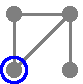
\includegraphics[scale=.6]{tubeB1}} & \raisebox{-.4cm}{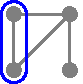
\includegraphics[scale=.6]{tubeB2}} & \raisebox{-.4cm}{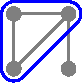
\includegraphics[scale=.6]{tubeB3}} & \raisebox{-.4cm}{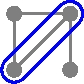
\includegraphics[scale=.6]{tubeB4}} & \raisebox{-.4cm}{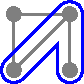
\includegraphics[scale=.6]{tubeB5}} & \raisebox{-.4cm}{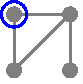
\includegraphics[scale=.6]{tubeB6}} & \raisebox{-.4cm}{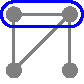
\includegraphics[scale=.6]{tubeB7}} & \raisebox{-.4cm}{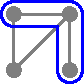
\includegraphics[scale=.6]{tubeB8}} & \raisebox{-.4cm}{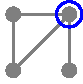
\includegraphics[scale=.6]{tubeB9}} & \raisebox{-.4cm}{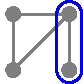
\includegraphics[scale=.6]{tubeB10}} & \raisebox{-.4cm}{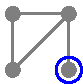
\includegraphics[scale=.6]{tubeB11}} \\[.6cm]
\text{$\b{g}$-vectors} & \compactVectorT{1}{0}{0} & \compactVectorT{0}{2}{0} & \compactVectorT{0}{0}{1} & \compactVectorT{1}{-2}{1} & \compactVectorT{1}{-2}{0} & \compactVectorT{-1}{2}{0} & \compactVectorT{-1}{0}{1} & \compactVectorT{-1}{0}{0} & \compactVectorT{0}{-2}{1} & \compactVectorT{0}{-2}{0} & \compactVectorT{0}{0}{-1} \\[.6cm]
\text{facet}		& -1 & 1 & -1 & 1 & 0 & 0 & 0 & 0 & 0 & 0 & 0 \\
\text{defining}		& 1 & -1 & 0 & 0 & 0 & 1 & 0 & 0 & 0 & 0 & 0 \\
\text{inequalities}	& 0 & 1 & -1 & 0 & 0 & -1 & 1 & 0 & 0 & 0 & 0 \\
					& 1 & 0 & 0 & -1 & 0 & 0 & 0 & 0 & 1 & 0 & 0 \\
					& 0 & 0 & -1 & 1 & 0 & 0 & 1 & 0 & -1 & 0 & 0 \\
					& 0 & 0 & 0 & 1 & -1 & 0 & 0 & 0 & -1 & 1 & 0 \\
					& 0 & 0 & 0 & 0 & 0 & 1 & -1 & 0 & 1 & 0 & 0 \\
					& 0 & 0 & 0 & 0 & 0 & 0 & 1 & -1 & -1 & 1 & 0 \\
					& 0 & 0 & 0 & 0 & 0 & 0 & 0 & 0 & 1 & -1 & 1 \\
					& 0 & 0 & 0 & 0 & 1 & 0 & 0 & 1 & 0 & -1 & 0 \\
					& 0 & 0 & 1 & 0 & 0 & 0 & -1 & 1 & 0 & 0 & 0 \\
					& 0 & 0 & 1 & -1 & 1 & 0 & 0 & 0 & 0 & 0 & 0 \\[.2cm]
\end{array}
\]

%sage: G = Graph([[1,2,3,4], [[1,2],[1,3],[2,3],[3,4]]])
%sage: M = Matrix([g_vector_GA(G, (1,)), g_vector_GA(G, (1,2)), g_vector_GA(G, (1,2,3)), [1,1,1,1]]).inverse()
%sage: rays = {tuple(tube) : (g_vector_GA(G, tube)*M)[:-1] for tube in tubes(G)}
%sage: rays
%{(1,): (1, 0, 0),
% (1, 2): (0, 1, 0),
% (1, 2, 3): (0, 0, 1),
% (1, 2, 3, 4): (0, 0, 0),
% (1, 3): (1/2, -1, 1/2),
% (1, 3, 4): (1, -2, 0),
% (2,): (-1, 2, 0),
% (2, 3): (-1/2, 0, 1/2),
% (2, 3, 4): (-1, 0, 0),
% (3,): (0, -2, 1),
% (3, 4): (0, -1, 0),
% (4,): (0, 0, -1)}

%sage: NF = Fan([Cone([rays[tuple(tube)] for tube in tubing]) for tubing in maximal_tubings(G)])
%sage: NF.rays()
%N( 1,  0,  0),
%N(-1,  2,  0),
%N( 0,  0,  1),
%N( 1, -2,  0),
%N( 0,  0, -1),
%N(-1,  0,  1),
%N( 1, -2,  1),
%N( 0, -2,  1),
%N(-1,  0,  0),
%N( 0,  1,  0),
%N( 0, -1,  0)
%in 3-d lattice N

%sage: TCNF = type_cone(NF)
%sage: TCNF
%A 11-dimensional polyhedron in QQ^11 defined as the convex hull of 1 vertex, 11 rays, 3 lines
%sage: TCNF.lines()
%(A line in the direction (0, 2, 0, -2, 0, 0, -2, -2, 0, 1, -1),
% A line in the direction (1, -1, 0, 1, 0, -1, 1, 0, -1, 0, 0),
% A line in the direction (1, -1, 1, 1, -1, 0, 2, 1, -1, 0, 0))
%sage: TCNF.inequalities()
%(An inequality (-1, 0, -1, 0, 0, 0, 1, 0, 0, 2, 0) x + 0 >= 0,
% An inequality (1, 1, 0, 0, 0, 0, 0, 0, 0, -2, 0) x + 0 >= 0,
% An inequality (0, -1, -1, 0, 0, 1, 0, 0, 0, 2, 0) x + 0 >= 0,
% An inequality (1, 0, 0, 0, 0, 0, -1, 1, 0, 0, 0) x + 0 >= 0,
% An inequality (0, 0, -1, 0, 0, 1, 1, -1, 0, 0, 0) x + 0 >= 0,
% An inequality (0, 0, 0, -1, 0, 0, 1, -1, 0, 0, 2) x + 0 >= 0,
% An inequality (0, 1, 0, 0, 0, -1, 0, 1, 0, 0, 0) x + 0 >= 0,
% An inequality (0, 0, 0, 0, 0, 1, 0, -1, -1, 0, 2) x + 0 >= 0,
% An inequality (0, 0, 0, 0, 1, 0, 0, 1, 0, 0, -2) x + 0 >= 0,
% An inequality (0, 0, 0, 1, 0, 0, 0, 0, 1, 0, -2) x + 0 >= 0,
% An inequality (0, 0, 1, 0, 0, -1, 0, 0, 1, 0, 0) x + 0 >= 0,
% An inequality (0, 0, 1, 1, 0, 0, -1, 0, 0, 0, 0) x + 0 >= 0)
%sage: len(TCNF.inequalities())
%12
\medskip
\end{example}

In the remaining of this section, we describe the facet-defining inequalities of the type cone of the graphical nested fans.
Observe first that we have already indirectly described this type cone when the graph is a path in \cref{prop:extremalExchangeablePairsAsso}.
Recall that on the path with~$n+1$ vertices, the tubes of the path are the intervals of~$[n+1]$ and that two intervals~$[i,j]$ and~$[i',j']$ of~$[n+1]$ are exchangeable if either~${i < i' \le j+1 < j'+1}$ or~${i' < i \le j'+1 < j+1}$.

\begin{proposition}
\label{prop:extremalExchangeablePairsA}
Two intervals~$[i,j]$ and~$[i',j']$ of~$[n+1]$ form an extremal exchangeable pair for the nested fan of the path if and only if~$i = i'+1$ and~$j = j'+1$, or the opposite.
\end{proposition}

We now consider an arbitrary graph~$\graphG$ and describe the type cone of its nested fan.
We give a necessary condition for an exchangeable pair to be extremal in \cref{lem:extremalExchangeablePairsGAonlyif}, exploit it in \cref{exm:constructionsGA}, and prove that it is actually a sufficient condition in \cref{prop:extremalExchangeablePairsGA}

\begin{lemma}
\label{lem:extremalExchangeablePairsGAonlyif}
If two tubes~$\tube$ and~$\tube'$ of~$\graphG$ form an extremal exchangeable pair for the nested fan of~$\graphG$, then~${\tube \ssm \{v\} = \tube' \ssm \{v'\}}$ for some neighbor~$v$ of~$\tube'$ and some neighbor~$v'$ of~$\tube$.
\end{lemma}

\begin{proof}
Consider an exchangeable pair~$\{\tube, \tube'\}$ of tubes of~$\graphG$.
The inner normal vector of the corresponding inequality of the type cone is
\[
\b{n}(\tube, \tube') \eqdef \b{f}_{\tube} + \b{f}_{\tube'} - \b{f}_{\tube\cup \tube'} - \sum_{\tube[s] \in \connectedComponents(\tube \cap \tube')} \b{f}_{\tube[s]}.
\]

By \cref{prop:exchangeablePairsGA}, $\tube'$ has a unique neighbor~$v$ in~$\tube \ssm \tube'$ and $\tube$ has a unique neighbor~$v'$ in~$\tube' \ssm \tube$.
Therefore, $\tube \ssm \tube'$ and~$\tube' \ssm \tube$ are both connected. Assume that $\tube \ssm \tube'\ne \{v\}$, and let $w\ne v$ be a non-disconnecting node of $\tube \ssm \tube'$. By \cref{prop:exchangeablePairsGA}, $\tilde \tube \eqdef \tube \ssm \{w\}$ and $\tube'$ are exchangeable, and $\tilde \tube' \eqdef (\tube \cup \tube') \ssm \{w\}$ and $\tube$ are exchangeable as well. Moreover, we have
\begin{align*}
\b{n}(\tilde \tube, \tube') + \b{n}( \tube, \tilde \tube')
& = \Big( \b{f}_{\tilde \tube} + \b{f}_{\tube'} - \b{f}_{\tilde \tube\cup \tube'} - \sum_{\tube[s] \in \connectedComponents(\tilde \tube \cap \tube')} \b{f}_{\tube[s]} \Big)
+ \Big( \b{f}_{\tube} + \b{f}_{\tilde \tube'} - \b{f}_{\tube\cup \tilde \tube'} - \sum_{\tube[s] \in \connectedComponents(\tube \cap \tilde \tube')} \b{f}_{\tube[s]} \Big) \\
& = \b{f}_{\tube} + \b{f}_{\tube'} - \b{f}_{\tube\cup \tube'} - \sum_{\tube[s] \in \connectedComponents(\tube \cap \tube')} \b{f}_{\tube[s]} =\b{n}(\tube, \tube'),
\end{align*}
as $\tilde \tube \cup \tube' = \tilde \tube'$, $\tilde \tube \cap \tube' = \tube \cap \tube'$, $\tube \cup \tilde \tube' = \tube \cup \tube'$ and $\connectedComponents(\tube \cap \tilde \tube') = \connectedComponents(\tilde \tube) = \tilde \tube$.
Therefore $\b{n}(\tube, \tube')$ defines a redundant inequality and $\{\tube, \tube'\}$ is not an extremal exchangeable pair.
The proof is symmetric if~$\tube' \ssm \tube \ne \{v'\}$.
\end{proof}

\begin{example}
\label{exm:constructionsGA}
We now exploit \cref{lem:extremalExchangeablePairsGAonlyif} to show that certain height functions belong to the type cone of~$\gvectorFan[\graphG]$ and recover the classical constructions of the graph associahedron.

\begin{enumerate}
\item Consider the height function~$\b{h} \in \R^{\tubes}$ given by~$\b{h}_{\tube} \eqdef -|\bigset{\tube[s] \in \tubes}{\tube[s] \subseteq \tube}|$. Then for any tubes~$\tube$ and~$\tube'$ such that ${\tube \ssm \{v\} = \tube' \ssm \{v'\}}$ for some neighbor~$v$ of~$\tube'$ and some neighbor~$v'$ of~$\tube$, we have
\[
\qquad\qquad
\dotprod{\b{n}(\tube, \tube')}{\b{h}} = |\bigset{\tube[s]\in\tubes}{\tube \symdif \tube' \subseteq \tube[s] \subseteq \tube \cup \tube'}|,
\]
where~$\tube \symdif \tube' = \{v,v'\}$ denotes the symmetric difference.
This quantity is positive since at least~$\tube \cup \tube'$ fulfills the condition.
Thus, the height function~$\b{h}$ belongs to the type cone~$\typeCone \big( \gvectorFan[\graphG] \big)$.
The polytope~$P_\b{h} \eqdef \set{\b{x} \in \R^\ground}{\dotprod{\gvector{\tube}}{\b{x}} \le \b{h}_{\tube} \text{ for any tube } \tube \in \tubes}$ is the graph associahedron constructed by A.~Postnikov's in~\cite{Postnikov}.
\item Consider now the height function~$\b{h} \in \R^{\tubes}$ given by~$\b{h}_{\tube} \eqdef -3^{|\tube|-2}$. Then for any tubes~$\tube$ and~$\tube'$ such that ${\tube \ssm \{v\} = \tube' \ssm \{v'\}}$ for some neighbor~$v$ of~$\tube'$ and some neighbor~$v'$ of~$\tube$, we have
\[
\qquad\qquad
\dotprod{\b{n}(\tube, \tube')}{\b{h}} = - 3^{|\tube|-2} - 3^{|\tube'|-2} + 3^{|\tube \cup \tube'|-2} + \sum_{\tube[s] \in \connectedComponents(\tube \cap \tube')} 3^{|\tube[s]|-2 } \ge - 2 \cdot 3^{|\tube \cup \tube'|-1} + 3^{|\tube \cup \tube'|} > 0.
\]
Thus, the height function~$\b{h}$ belongs to the type cone~$\typeCone \big( \gvectorFan[\graphG] \big)$.
The corresponding polytope~$P_\b{h}$ is the graph associahedron constructed by S.~Devadoss's in~\cite{Devadoss}.
\item Finally, consider the height function~$\b{h} \in \R^{\tubes}$ given by~$\b{h}_{\tube} \eqdef |\bigset{\tube[s] \in \tubes}{\tube[s] \supseteq \tube}|$. Then for any tubes~$\tube$ and~$\tube'$ such that ${\tube \ssm \{v\} = \tube' \ssm \{v'\}}$ for some neighbor~$v$ of~$\tube'$ and some neighbor~$v'$ of~$\tube$, we have
\begin{align*}
\qquad\qquad
\dotprod{\b{n}(\tube, \tube')}{\b{h}} = \; & |\bigset{(\tube[r], \tube[s]) \in \tubes \times \connectedComponents(\tube \cap \tube')}{\tube[s] \subseteq \tube[r] \text{ and } \tube, \tube' \not\subseteq \tube[r]}| \\
& + \big( |\connectedComponents(\tube \cap \tube')|-1 \big) \cdot | \bigset{\tube[r] \in \tubes}{\tube \text{ or } \tube'\subseteq \tube[r]}\big|.
\end{align*}
Any connected component of~$\tube \cap \tube'$ certifies the positivity of this evaluation, showing that the height function~$\b{h}$ belongs to~$\typeCone \big( \gvectorFan[\graphG] \big)$. The corresponding realization~$P_\b{h}$ of the graph associahedron is new, to the best of our knowledge. 
\end{enumerate}
\end{example}

We now show that the condition of \cref{lem:extremalExchangeablePairsGAonlyif} actually characterizes the extremal exchangeable pairs of the nested fan~$\gvectorFan[\graphG]$.

\begin{proposition}
\label{prop:extremalExchangeablePairsGA}
Two tubes~$\tube$ and~$\tube'$ of~$\graphG$ form an extremal exchangeable pair for the nested fan of~$\graphG$ if and only if~${\tube \ssm \{v\} = \tube' \ssm \{v'\}}$ for some neighbor~$v$ of~$\tube'$ and some neighbor~$v'$ of~$\tube$.
\end{proposition}

\begin{proof}
By \cref{lem:extremalExchangeablePairsGAonlyif}, an exchangeable pair $\{\tube, \tube'\}$ is not extremal unless both $\tube \ssm \tube'$ and $\tube' \ssm \tube$ are singletons. We now need to show that all these pairs are extremal. Until we finish the proof, we will call such a pair a \defn{suspected extremal pair}.

Let $\{\tube, \tube'\}$ be a suspected extremal pair.
To prove that it is extremal, we will construct a vector $\b{w} \in \R^{\tubes}$ such that $\dotprod{\b{n}(\tube, \tube')}{\b{w}}< 0,$
but $\dotprod{\b{n}(\tilde \tube, \tilde \tube')}{\b{w}}>0$ for any other suspected extremal pair $\{\tilde \tube, \tilde \tube'\}$. This will show that the inequality induced by~$\{\tube, \tube'\}$ is not redundant.

Define $\alpha(\tube,\tube') \eqdef \set{\tube[r] \in \tubes}{\tube \symdif \tube' \subseteq \tube[r] \subseteq \tube \cup \tube'}$, where $\symdif$ denotes the symmetric difference, and define $\b{x} \in \R^{\tubes}$ be such that
\[
\b{x}_{\tube[s]} = -|\bigset{\tube[r] \in \tubes \ssm \alpha(\tube, \tube')}{\tube[r] \subseteq \tube[s]}|
\]
for each tube~$\tube[s] \in \tubes$.
For any suspected extremal pair $\{\tilde \tube, \tilde \tube'\}$ we have
\[
\dotprod{\b{n}(\tilde \tube, \tilde \tube')}{\b{x}} = |\alpha(\tilde \tube, \tilde \tube')\ssm \alpha(\tube, \tube')| \ge 0.
\]
Notice that $\dotprod{\b{n}(\tilde \tube, \tilde \tube')}{\b{x}} = 0$ if $\alpha(\tilde \tube, \tilde \tube') \subseteq \alpha(\tube,\tube')$ and $\dotprod{\b{n}(\tilde \tube, \tilde \tube')}{\b{x}} \ge 1$ otherwise.
In particular, if $\{\tilde \tube, \tilde \tube'\} \ne \{\tube, \tube'\}$ then $\dotprod{\b{n}(\tilde \tube, \tilde \tube')}{\b{x}} \ge 1$ unless $\tilde \tube \cup \tilde \tube' \subsetneq \tube \cup \tube'$ because $\tilde \tube \cup \tilde \tube' \in \alpha(\tilde \tube, \tilde \tube')$, and if $\tilde \tube \cup \tilde \tube' = \tube \cup \tube'$ but $\{\tilde \tube, \tilde \tube'\} \ne \{\tube, \tube'\}$, then either $\tube$ or $\tube'$ will belong to $\alpha(\tilde \tube, \tilde \tube')$. 

Now, define $\b{y}\in\R^{\tubes}$ by
\[
\b{y}_{\tube[s]} = \begin{cases}
	-1 & \text{ if } |\tube[s]| \ge |\tube|, \\
	0 & \text{ otherwise},
\end{cases}
\]
for each tube~$\tube[s] \in \tubes$.
We have $\dotprod{\b{n}(\tube, \tube')}{\b{y}} = -1$. For any suspected extremal pair $\{\tilde \tube, \tilde \tube'\}$ we have $\dotprod{\b{n}(\tilde \tube, \tilde \tube')}{\b{y}} \ge -1$. If moreover $\tilde \tube \cup \tilde \tube' \subsetneq \tube \cup \tube'$, then we have $\dotprod{\b{n}(\tilde \tube, \tilde \tube')}{\b{y}} \ge 0$. 

Finally, consider $\b{z} \in \R^{\tubes}$ given by
\[
\b{z}_{\tube[s]} = -|\bigset{\tube[r] \in \alpha(\tube, \tube')}{\tube[r] \subseteq \tube[s]}|,
\]
for each tube~$\tube[s] \in \tubes$.
It verifies $\dotprod{\b{n}(\tilde \tube, \tilde \tube')}{\b{z}} \ge 0$ for any suspected extremal pair~$\{\tilde \tube, \tilde \tube'\}$, and $\dotprod{\b{n}(\tilde \tube, \tilde \tube')}{\b{z}} = |\alpha(\tilde \tube, \tilde \tube')| > 0$ if $\alpha(\tilde \tube, \tilde \tube') \subseteq \alpha(\tube, \tube')$.

For $0 < \varepsilon < 1$, and $0 < \delta < \frac{\varepsilon}{|\alpha(\tube, \tube')|}$, we claim that the vector $\b{w} \eqdef \b{x} + \varepsilon \b{y} + \delta \b{z}$ fulfills the desired properties.
Indeed, if $\{\tilde \tube, \tilde \tube'\} \ne \{\tube,\tube'\}$ is a suspected extremal pair with $\alpha(\tilde \tube, \tilde \tube') \not \subseteq \alpha(\tube,\tube')$, then 
\[
\dotprod{\b{n}(\tilde \tube, \tilde \tube')}{\b{w}} = \underbrace{\dotprod{\b{n}(\tilde \tube, \tilde \tube')}{\b{x}}}_{\ge 1} + \underbrace{\varepsilon \dotprod{\b{n}(\tilde \tube, \tilde \tube')}{\b{y}}}_{> -1} + \underbrace{\delta \dotprod{\b{n}(\tilde \tube, \tilde \tube')}{\b{z}}}_{\ge 0} > 0.
\]
If $\{\tilde \tube, \tilde \tube'\} \ne \{\tube,\tube'\}$ is a suspected extremal pair with $\alpha(\tilde \tube, \tilde \tube') \subseteq \alpha(\tube,\tube')$, then $\tilde \tube \cup \tilde \tube' \subsetneq \tube \cup \tube'$ and 
\[
\dotprod{\b{n}(\tilde \tube, \tilde \tube')}{\b{w}} = \underbrace{\dotprod{\b{n}(\tilde \tube, \tilde \tube')}{\b{x}}}_{= 0} + \underbrace{\varepsilon \dotprod{\b{n}(\tilde \tube, \tilde \tube')}{\b{y}}}_{\ge 0} + \underbrace{\delta \dotprod{\b{n}(\tilde \tube, \tilde \tube')}{\b{z}}}_{> 0} > 0.
\]
However,
\[
\dotprod{\b{n}(\tube, \tube')}{\b{w}} = \underbrace{\dotprod{\b{n}(\tube, \tube')}{\b{x}}}_{= 0} + \underbrace{\varepsilon \dotprod{\b{n}(\tube, \tube')}{\b{y}}}_{= -\varepsilon} + \underbrace{\delta \dotprod{\b{n}( \tube,  \tube')}{\b{z}}}_{= \delta |\alpha(\tube ,\tube')| < \varepsilon} < 0.
\qedhere
\]
\end{proof}

The following statement reformulates \cref{prop:extremalExchangeablePairsGA}.

\begin{corollary}
\label{coro:extremalExchangeablePairsGA}
The extremal exchangeable pairs for the nested fan of~$\graphG$ are precisely the pairs of tubes~${\tube[s] \ssm \{v'\}}$ and~${\tube[s] \ssm \{v\}}$ for any tube~$\tube[s] \in \tubes$ and distinct non-disconnecting vertices~$v,v'$~of~$\tube[s]$.
\end{corollary}

\enlargethispage{-.1cm}
We derive from \cref{prop:extremalExchangeablePairsGA} and \cref{coro:extremalExchangeablePairsGA} all polytopal realizations of the nested fan.

\begin{corollary}
\label{coro:typeconenestedfan}
Consider a graph~$\graphG$ on~$\ground$ with tubes~$\tubes$. 
Then, for a height vector~$\b{h} \in \R^{\tubes}$, the nested fan~$\gvectorFan[\graphG]$ is the normal fan of the graph associahedron
\[
\set{\b{x} \in \R^\ground}{\dotprod{\gvector{\tube}}{\b{x}} \le \b{h}_{\tube} \text{ for any tube } \tube \in \tubes}
\]
if and only if~$\b{h}_{\varnothing} = \b{h}_{\graphG} = 0$ and
 $\b{h}_{\tube[s] \ssm \{v'\}} + \b{h}_{\tube[s] \ssm \{v\}} > \b{h}_{\tube[s]} + \b{h}_{\tube[s] \ssm \{v, v'\}}$ for any tube~$\tube[s] \in \tubes$ and distinct non-disconnecting vertices~$v,v'$ of~$\tube[s]$.
\end{corollary}

We also obtain from \cref{prop:extremalExchangeablePairsGA} the following surprising property.

\begin{corollary}
Any $\b{c}$-vector supports at least one extremal exchangeable pair.
\end{corollary}

\begin{proof}
Consider a $\b{c}$-vector~$\b{e}_v - \b{e}_{v'}$ for two distinct vertices~$v, v'$ in a common connected component of~$\graphG$. Let~$\tube[r]$ be a path from~$v$ to~$v'$ in~$\graphG$ and let~$\tube \eqdef \tube[r] \cup \{v\}$ and~$\tube' \eqdef \tube[r] \cup \{v'\}$. Then $\{\tube, \tube'\}$ is an extremal exchangeable pair with $\b{c}$-vector~$\b{e}_v - \b{e}_{v'}$.
\end{proof}

We derive from \cref{coro:extremalExchangeablePairsGA} the number of extremal exchangeable pairs of the nested fan.
For a tube~$\tube$ of~$\graphG$, we denote by~$\nonDisconnecting(\tube)$ the number of non-disconnecting vertices of~$\tube$.
In other words, $\nonDisconnecting(\tube)$ is the number of tubes covered by~$\tube$ in the inclusion poset of all tubes of~$\graphG$.

\begin{corollary}
\label{coro:numberExtremalExchangeablePairsGA}
The nested fan~$\gvectorFan[\graphG]$ has~$\!\!\!\! \sum\limits_{\tube[s] \in \tubes} \!\! \binom{\nonDisconnecting(\tube[s])}{2}$ extremal exchangeable pairs.
\end{corollary}

The formula of \cref{coro:numberExtremalExchangeablePairsGA} can be made more explicit for specific families of graph associahedra discussed in the introduction and illustrated in \cref{fig:specialGraphAssociahedra}.

\begin{proposition}
The number of extremal exchangeable pairs of the nested fan~$\gvectorFan[\graphG]$ is:
\begin{itemize}
\item $2^{n-2}\binom{n}{2}$ for the permutahedron (complete graph associahedron),
\item $\binom{n}{2}$ for the associahedron (path associahedron),
\item $3\binom{n}{2} - n$ for the cyclohedron (cycle associahedron),
\item $n-1+2^{n-3}\binom{n-1}{2}$ for the stellohedron (star associahedron).
\end{itemize}
\end{proposition}

\begin{proof}
For the permutahedron, choose any two vertices~$v,v'$, and complete them into a tube by selecting any subset of the~$n-2$ remaining vertices.
For the associahedron, choose any two vertices~$v,v'$, and complete them into a tube by taking the path between them.
For the cyclohedron, choose the two vertices~$v,v'$, and complete them into a tube by taking either all the cycle, or one of the two paths between~$v$ and~$v'$ (this gives three options in general, but only two when~$v,v'$ are neighbors).
For the stellohedron, choose either~$v$ as the center of the star and~$v'$ as one of the $n-1$ leaves, or $v$~and~$v'$ as leaves of the star and complete them into a tube by taking the center and any subset of the $n-3$ remaining leaves.
\end{proof}

To conclude on graph associahedra, we characterize the graphs~$\graphG$ whose nested fan has a simplicial type cone.

\begin{proposition}\label{prop:simplicialnestedfan}
The type cone~$\typeCone \big( \gvectorFan[\graphG] \big)$ is simplicial if and only if~$\graphG$ is a path.
\end{proposition}

\begin{proof}
Note that any tube~$\tube$ with~$|\tube| \ge 2$ has two non-disconnecting vertices when it is a path, and at least three non-disconnecting vertices otherwise (the leaves of an arbitrary spanning tree of~$\tube$, or any vertex if it is a cycle).
Therefore, each tube of~$\tubes$ which is not a singleton contributes to at least one extremal exchangeable pair.
We conclude that the number of extremal exchangeable pairs is at least:
\[
|\tubes| - |V| = |\tubes \ssm \{\varnothing, \graphG\}| - (|V|-1) = N - n,
\]
with equality if and only if all tubes of~$\graphG$ are paths, \ie if and only if~$\graphG$ is a path.
\end{proof}

%%%%%%%%%%%%%%%%%%%%%%%%%%%%%%%%%%%%%%%

\addtocontents{toc}{\vspace{.1cm}}
\section*{Acknowledgments}


%%%%%%%%%%%%%%%%%%%%%%%%%%%%%%%%%%%%%%%

\newpage
\bibliographystyle{alpha}
\bibliography{typeConeGraphAssociahedra}
\label{sec:biblio}

\end{document}
